% Options for packages loaded elsewhere
\PassOptionsToPackage{unicode}{hyperref}
\PassOptionsToPackage{hyphens}{url}
\documentclass[
  ignorenonframetext,
]{beamer}
\newif\ifbibliography
\usepackage{pgfpages}
\setbeamertemplate{caption}[numbered]
\setbeamertemplate{caption label separator}{: }
\setbeamercolor{caption name}{fg=normal text.fg}
\beamertemplatenavigationsymbolsempty
% remove section numbering
\setbeamertemplate{part page}{
  \centering
  \begin{beamercolorbox}[sep=16pt,center]{part title}
    \usebeamerfont{part title}\insertpart\par
  \end{beamercolorbox}
}
\setbeamertemplate{section page}{
  \centering
  \begin{beamercolorbox}[sep=12pt,center]{section title}
    \usebeamerfont{section title}\insertsection\par
  \end{beamercolorbox}
}
\setbeamertemplate{subsection page}{
  \centering
  \begin{beamercolorbox}[sep=8pt,center]{subsection title}
    \usebeamerfont{subsection title}\insertsubsection\par
  \end{beamercolorbox}
}
% Prevent slide breaks in the middle of a paragraph
\widowpenalties 1 10000
\raggedbottom
\AtBeginPart{
  \frame{\partpage}
}
\AtBeginSection{
  \ifbibliography
  \else
    \frame{\sectionpage}
  \fi
}
\AtBeginSubsection{
  \frame{\subsectionpage}
}
\usepackage{iftex}
\ifPDFTeX
  \usepackage[T1]{fontenc}
  \usepackage[utf8]{inputenc}
  \usepackage{textcomp} % provide euro and other symbols
\else % if luatex or xetex
  \usepackage{unicode-math} % this also loads fontspec
  \defaultfontfeatures{Scale=MatchLowercase}
  \defaultfontfeatures[\rmfamily]{Ligatures=TeX,Scale=1}
\fi
\usepackage{lmodern}
\ifPDFTeX\else
  % xetex/luatex font selection
\fi
% Use upquote if available, for straight quotes in verbatim environments
\IfFileExists{upquote.sty}{\usepackage{upquote}}{}
\IfFileExists{microtype.sty}{% use microtype if available
  \usepackage[]{microtype}
  \UseMicrotypeSet[protrusion]{basicmath} % disable protrusion for tt fonts
}{}
\makeatletter
\@ifundefined{KOMAClassName}{% if non-KOMA class
  \IfFileExists{parskip.sty}{%
    \usepackage{parskip}
  }{% else
    \setlength{\parindent}{0pt}
    \setlength{\parskip}{6pt plus 2pt minus 1pt}}
}{% if KOMA class
  \KOMAoptions{parskip=half}}
\makeatother
\usepackage{longtable,booktabs,array}
\newcounter{none} % for unnumbered tables
\usepackage{calc} % for calculating minipage widths
\usepackage{caption}
% Make caption package work with longtable
\makeatletter
\def\fnum@table{\tablename~\thetable}
\makeatother
\usepackage{graphicx}
\makeatletter
\newsavebox\pandoc@box
\newcommand*\pandocbounded[1]{% scales image to fit in text height/width
  \sbox\pandoc@box{#1}%
  \Gscale@div\@tempa{\textheight}{\dimexpr\ht\pandoc@box+\dp\pandoc@box\relax}%
  \Gscale@div\@tempb{\linewidth}{\wd\pandoc@box}%
  \ifdim\@tempb\p@<\@tempa\p@\let\@tempa\@tempb\fi% select the smaller of both
  \ifdim\@tempa\p@<\p@\scalebox{\@tempa}{\usebox\pandoc@box}%
  \else\usebox{\pandoc@box}%
  \fi%
}
% Set default figure placement to htbp
\def\fps@figure{htbp}
\makeatother
\setlength{\emergencystretch}{3em} % prevent overfull lines
\providecommand{\tightlist}{%
  \setlength{\itemsep}{0pt}\setlength{\parskip}{0pt}}
\usepackage{bookmark}
\IfFileExists{xurl.sty}{\usepackage{xurl}}{} % add URL line breaks if available
\urlstyle{same}
\hypersetup{
  hidelinks,
  pdfcreator={LaTeX via pandoc}}

\author{\texorpdfstring{}{}}
\date{}

\begin{document}

\begin{frame}[fragile]{Results}
\protect\phantomsection\label{results}
The Docxology Template was evaluated through a multi-project pipeline
execution, measuring test coverage, pipeline timing, output integrity,
and steganographic performance across three heterogeneous exemplar
projects.

\begin{block}{Multi-Project Pipeline Execution}
\protect\phantomsection\label{multi-project-pipeline-execution}
All three projects were executed through the full eight-stage pipeline
using the \texttt{run.sh} interactive orchestrator with the ``all
projects core (fast)'' configuration, which skips infrastructure tests
and LLM review to isolate project-level performance.

{\def\LTcaptype{none} % do not increment counter
\begin{longtable}[]{@{}lllll@{}}
\toprule\noalign{}
Project & Stages & Duration & Tests & Coverage \\
\midrule\noalign{}
\endhead
\texttt{code\_project} & 7 & 43.4s & 58/58 & 96.6\% \\
\texttt{cognitive\_case\_diagrams} & 7 & 56.0s & 257/257 &
\textasciitilde96\% \\
\texttt{template} & 7 & 22.6s & 36/36 & 90\%+ \\
\bottomrule\noalign{}
\end{longtable}
}

\textbf{Overall success rate}: 100.0\% (3/3 projects) \textbf{Total
pipeline duration}: 121.9s \textbf{Average per project}: 40.6s

The \texttt{cognitive\_case\_diagrams} project, with its 257 tests and
25+ programmatically generated figures via 17 DisCoPy renderers,
represents the most computationally intensive exemplar---yet completes
in under one minute.
\end{block}

\begin{block}{Infrastructure Test Suite}
\protect\phantomsection\label{infrastructure-test-suite}
The infrastructure layer is validated by a separate test suite of
significant scale:

{\def\LTcaptype{none} % do not increment counter
\begin{longtable}[]{@{}ll@{}}
\toprule\noalign{}
Metric & Value \\
\midrule\noalign{}
\endhead
Test files & 148 \\
Total tests & 3,053 \\
Infrastructure coverage threshold & 60\% (achieved: 83\%+) \\
Zero-mock violations & 0 \\
Real filesystem operations & ✓ \\
Real subprocess invocations & ✓ \\
\bottomrule\noalign{}
\end{longtable}
}

This test suite exercises all ten infrastructure modules, including the
rendering pipeline (Pandoc/XeLaTeX integration), steganographic
operations (alpha-channel overlay, QR injection), and LLM client
interactions (real HTTP calls to Ollama).
\end{block}

\begin{block}{Infrastructure Module Inventory}
\protect\phantomsection\label{infrastructure-module-inventory}
The introspection module (\texttt{template.introspection})
programmatically enumerates the infrastructure layer, confirming the
following module distribution:

{\def\LTcaptype{none} % do not increment counter
\begin{longtable}[]{@{}
  >{\raggedright\arraybackslash}p{(\linewidth - 8\tabcolsep) * \real{0.1250}}
  >{\centering\arraybackslash}p{(\linewidth - 8\tabcolsep) * \real{0.2031}}
  >{\centering\arraybackslash}p{(\linewidth - 8\tabcolsep) * \real{0.2344}}
  >{\centering\arraybackslash}p{(\linewidth - 8\tabcolsep) * \real{0.2344}}
  >{\raggedright\arraybackslash}p{(\linewidth - 8\tabcolsep) * \real{0.2031}}@{}}
\toprule\noalign{}
\begin{minipage}[b]{\linewidth}\raggedright
Module
\end{minipage} & \begin{minipage}[b]{\linewidth}\centering
Python Files
\end{minipage} & \begin{minipage}[b]{\linewidth}\centering
Has AGENTS.md
\end{minipage} & \begin{minipage}[b]{\linewidth}\centering
Has README.md
\end{minipage} & \begin{minipage}[b]{\linewidth}\raggedright
Key Exports
\end{minipage} \\
\midrule\noalign{}
\endhead
\texttt{core} & 28 & ✓ & ✓ & \texttt{get\_logger},
\texttt{load\_config}, \texttt{TemplateError} \\
\texttt{documentation} & 6 & ✓ & ✓ & \texttt{FigureManager},
\texttt{generate\_glossary} \\
\texttt{llm} & 30 & ✓ & ✓ & LLM review, literature search,
translation \\
\texttt{project} & 2 & ✓ & ✓ & \texttt{\_discover\_project}, workspace
management \\
\texttt{publishing} & 9 & ✓ & ✓ & Citation generation (APA, BibTeX,
MLA), Zenodo \\
\texttt{rendering} & 12 & ✓ & ✓ & PDF rendering, Pandoc filters, HTML
reports \\
\texttt{reporting} & 14 & ✓ & ✓ & Coverage parsing, executive reports \\
\texttt{scientific} & 6 & ✓ & ✓ & \texttt{check\_numerical\_stability},
\texttt{benchmark\_function} \\
\texttt{steganography} & 8 & ✓ & ✓ & Metadata injection, QR overlays,
hashing \\
\texttt{validation} & 22 & ✓ & ✓ & PDF validation, Markdown checking,
CLI \\
\textbf{Total} & \textbf{137} & \textbf{10/10} & \textbf{10/10} & \\
\bottomrule\noalign{}
\end{longtable}
}

All ten modules have complete documentation coverage (both
\texttt{AGENTS.md} and \texttt{README.md}), confirming the Documentation
Duality standard.
\end{block}

\begin{block}{Pipeline Stage Execution}
\protect\phantomsection\label{pipeline-stage-execution}
The eight pipeline stages execute sequentially with strict error
propagation:

{\def\LTcaptype{none} % do not increment counter
\begin{longtable}[]{@{}
  >{\raggedright\arraybackslash}p{(\linewidth - 6\tabcolsep) * \real{0.1591}}
  >{\raggedright\arraybackslash}p{(\linewidth - 6\tabcolsep) * \real{0.1818}}
  >{\raggedright\arraybackslash}p{(\linewidth - 6\tabcolsep) * \real{0.3409}}
  >{\raggedright\arraybackslash}p{(\linewidth - 6\tabcolsep) * \real{0.3182}}@{}}
\toprule\noalign{}
\begin{minipage}[b]{\linewidth}\raggedright
Stage
\end{minipage} & \begin{minipage}[b]{\linewidth}\raggedright
Script
\end{minipage} & \begin{minipage}[b]{\linewidth}\raggedright
Responsibility
\end{minipage} & \begin{minipage}[b]{\linewidth}\raggedright
Failure Mode
\end{minipage} \\
\midrule\noalign{}
\endhead
00 & \texttt{00\_setup\_environment.py} & Environment validation & Hard
fail \\
01 & \texttt{01\_run\_tests.py} & Test execution + coverage &
Configurable tolerance \\
02 & \texttt{02\_run\_analysis.py} & Script invocation & Hard fail \\
03 & \texttt{03\_render\_pdf.py} & Pandoc + XeLaTeX & Hard fail \\
04 & \texttt{04\_validate\_output.py} & PDF integrity & Warning +
report \\
05 & \texttt{05\_copy\_outputs.py} & Output organization & Soft fail \\
06 & \texttt{06\_llm\_review.py} & LLM-assisted review & Skippable \\
07 & \texttt{07\_generate\_executive\_report.py} & Report aggregation &
Soft fail \\
\bottomrule\noalign{}
\end{longtable}
}
\end{block}

\begin{block}{Steganographic Performance}
\protect\phantomsection\label{steganographic-performance}
The steganography subsystem (\texttt{infrastructure.steganography}) was
benchmarked across all three project PDFs:

{\def\LTcaptype{none} % do not increment counter
\begin{longtable}[]{@{}
  >{\raggedright\arraybackslash}p{(\linewidth - 12\tabcolsep) * \real{0.1500}}
  >{\centering\arraybackslash}p{(\linewidth - 12\tabcolsep) * \real{0.1167}}
  >{\centering\arraybackslash}p{(\linewidth - 12\tabcolsep) * \real{0.1667}}
  >{\centering\arraybackslash}p{(\linewidth - 12\tabcolsep) * \real{0.1500}}
  >{\centering\arraybackslash}p{(\linewidth - 12\tabcolsep) * \real{0.1500}}
  >{\centering\arraybackslash}p{(\linewidth - 12\tabcolsep) * \real{0.1500}}
  >{\centering\arraybackslash}p{(\linewidth - 12\tabcolsep) * \real{0.1167}}@{}}
\toprule\noalign{}
\begin{minipage}[b]{\linewidth}\raggedright
Project
\end{minipage} & \begin{minipage}[b]{\linewidth}\centering
Pages
\end{minipage} & \begin{minipage}[b]{\linewidth}\centering
Metadata
\end{minipage} & \begin{minipage}[b]{\linewidth}\centering
SHA-256
\end{minipage} & \begin{minipage}[b]{\linewidth}\centering
Overlay
\end{minipage} & \begin{minipage}[b]{\linewidth}\centering
QR Code
\end{minipage} & \begin{minipage}[b]{\linewidth}\centering
Total
\end{minipage} \\
\midrule\noalign{}
\endhead
\texttt{code\_project} & 20 & \textless{} 0.3s & \textless{} 0.05s &
\textless{} 0.8s & \textless{} 0.4s & \textless{} 1.5s \\
\texttt{cognitive\_case\_diagrams} & 77 & \textless{} 0.3s & \textless{}
0.05s & \textless{} 2.0s & \textless{} 0.4s & \textless{} 2.8s \\
\texttt{template} & 5 & \textless{} 0.3s & \textless{} 0.05s &
\textless{} 0.3s & \textless{} 0.4s & \textless{} 1.0s \\
\bottomrule\noalign{}
\end{longtable}
}

The steganographic watermark survives standard PDF operations (viewing,
printing) but is detectable through pixel-level analysis of the alpha
channel. Performance scales linearly with page count, dominated by the
alpha-channel overlay phase.
\end{block}

\begin{block}{Self-Referential Analysis}
\protect\phantomsection\label{self-referential-analysis}
This manuscript is itself a product of the template pipeline,
demonstrating its self-referential capability. The \texttt{template}
project's \texttt{src/template/introspection.py} module programmatically
analyzes the repository and generates three architecture figures:

\pandocbounded{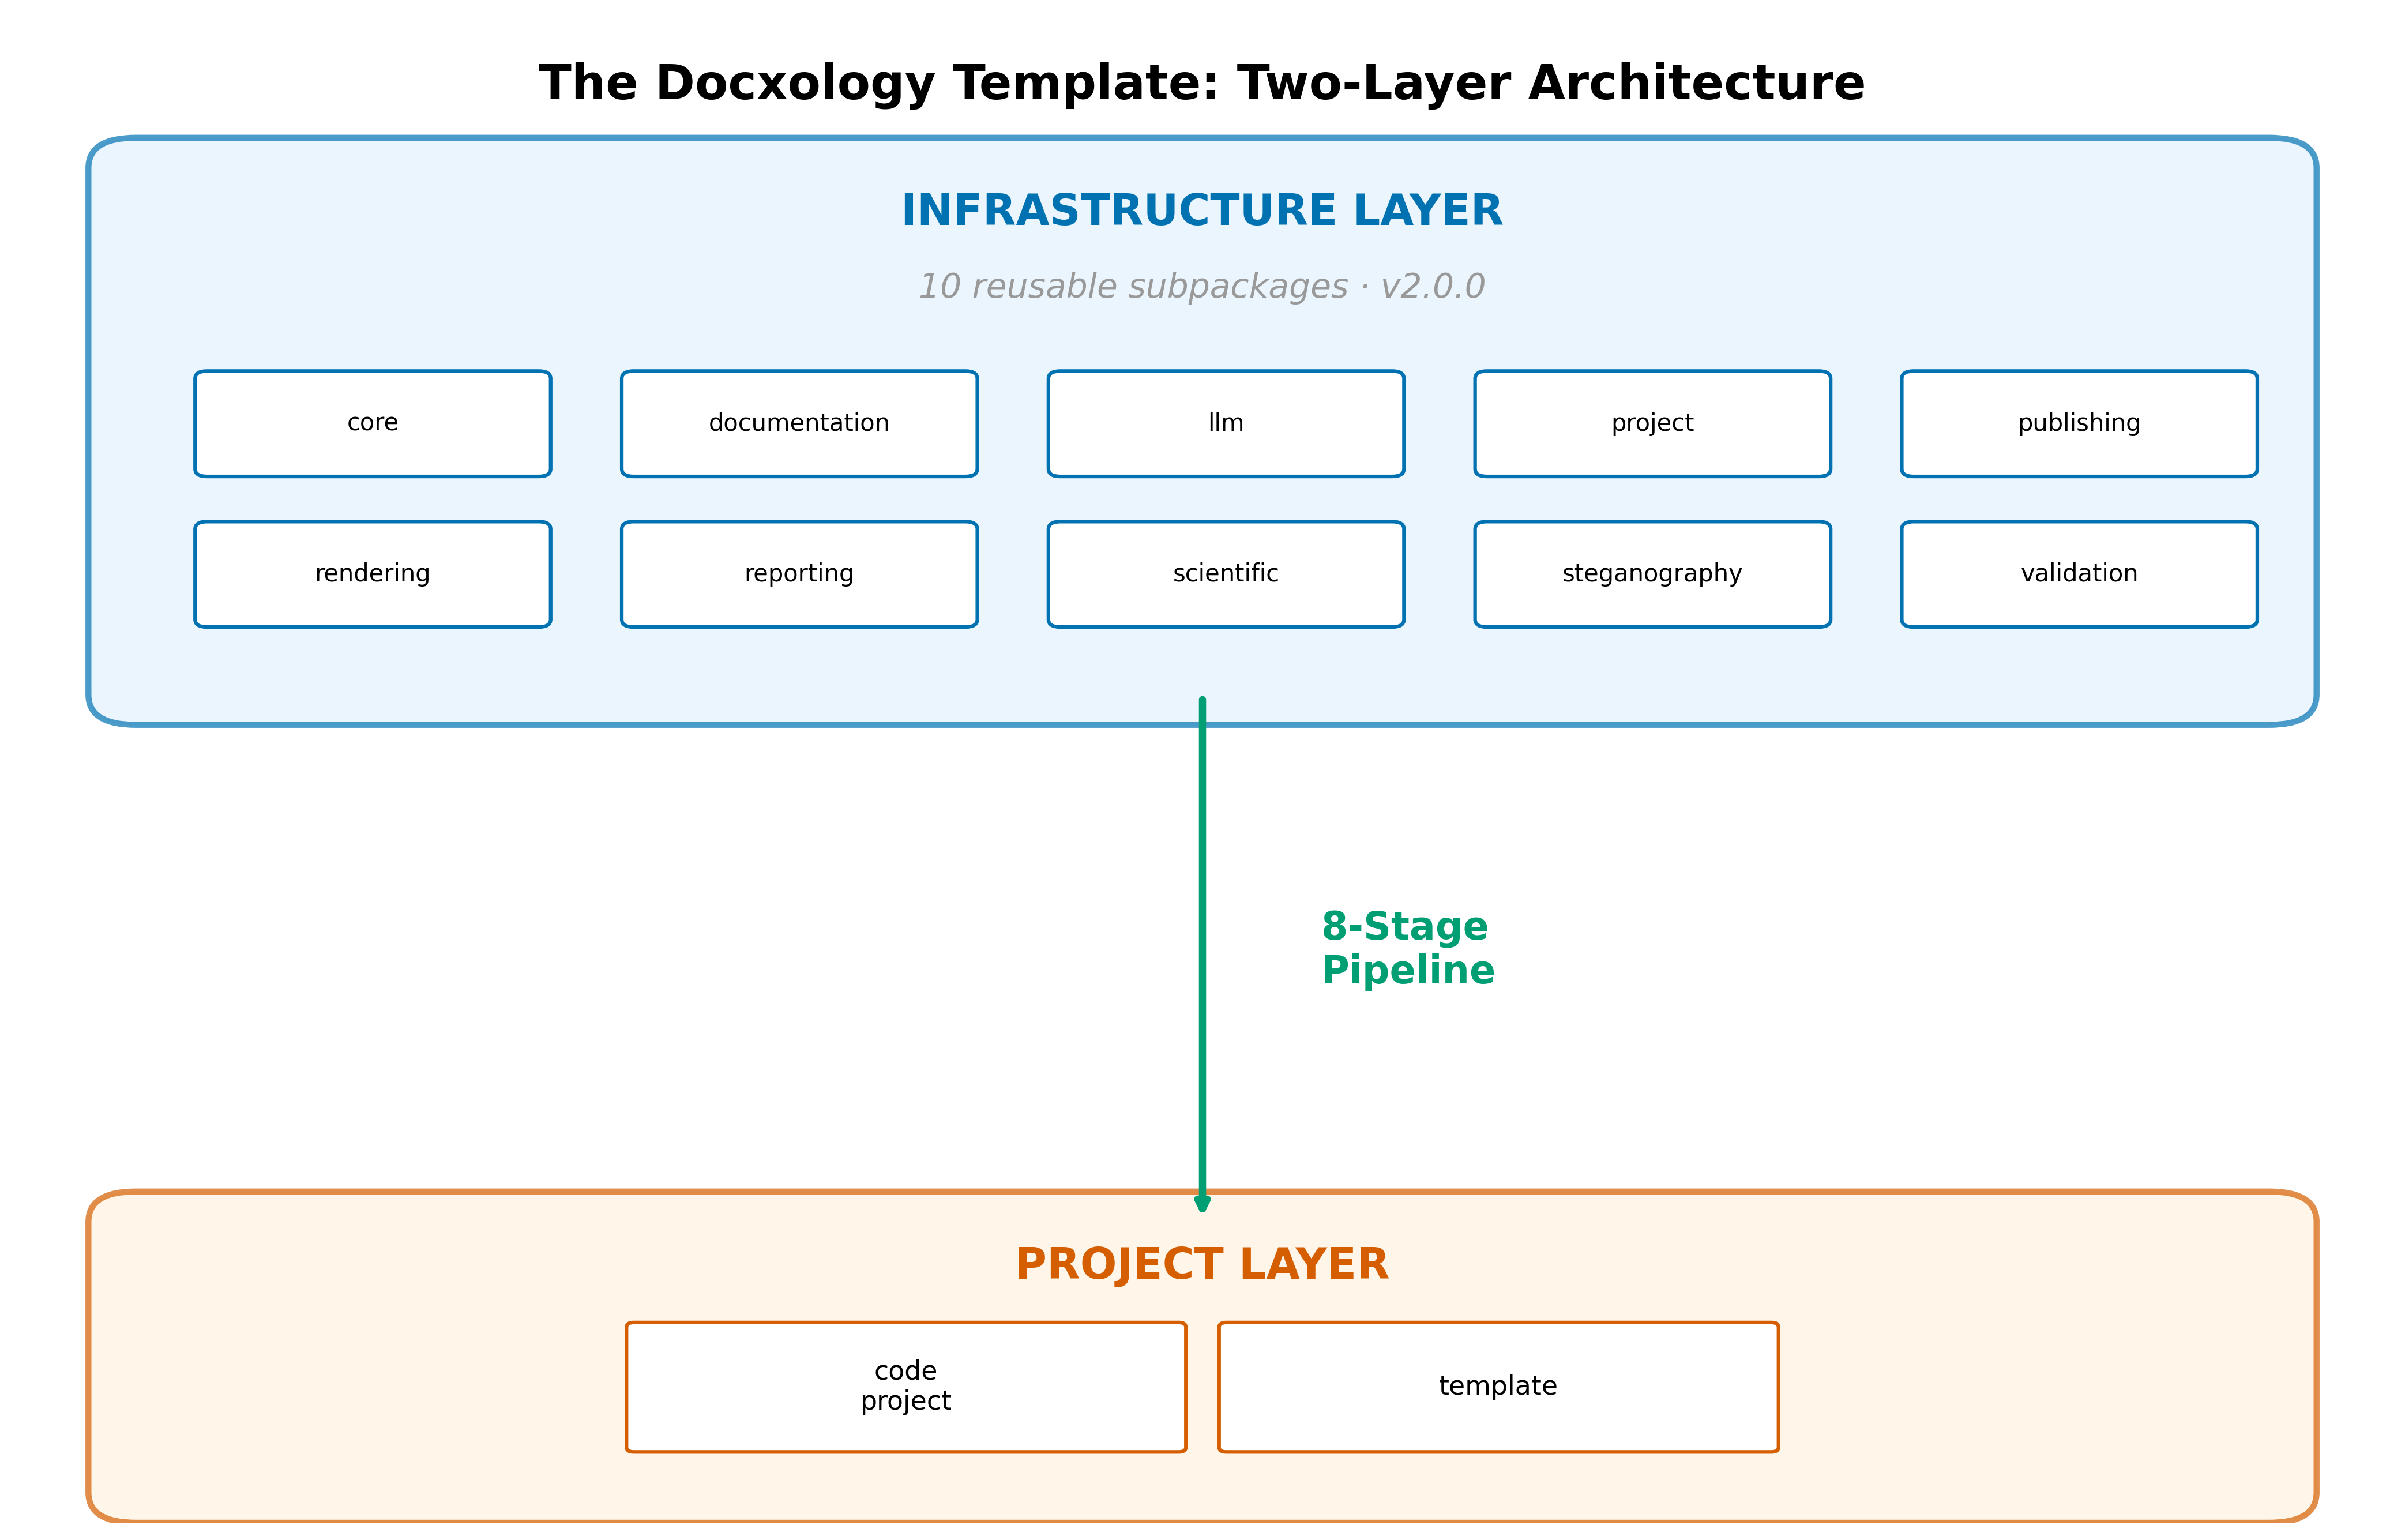
\includegraphics[keepaspectratio,alt={Two-Layer Architecture Overview}]{../figures/architecture_overview.png}}
\emph{Figure 1: The Two-Layer Architecture separating infrastructure
modules from project workspaces.}

\pandocbounded{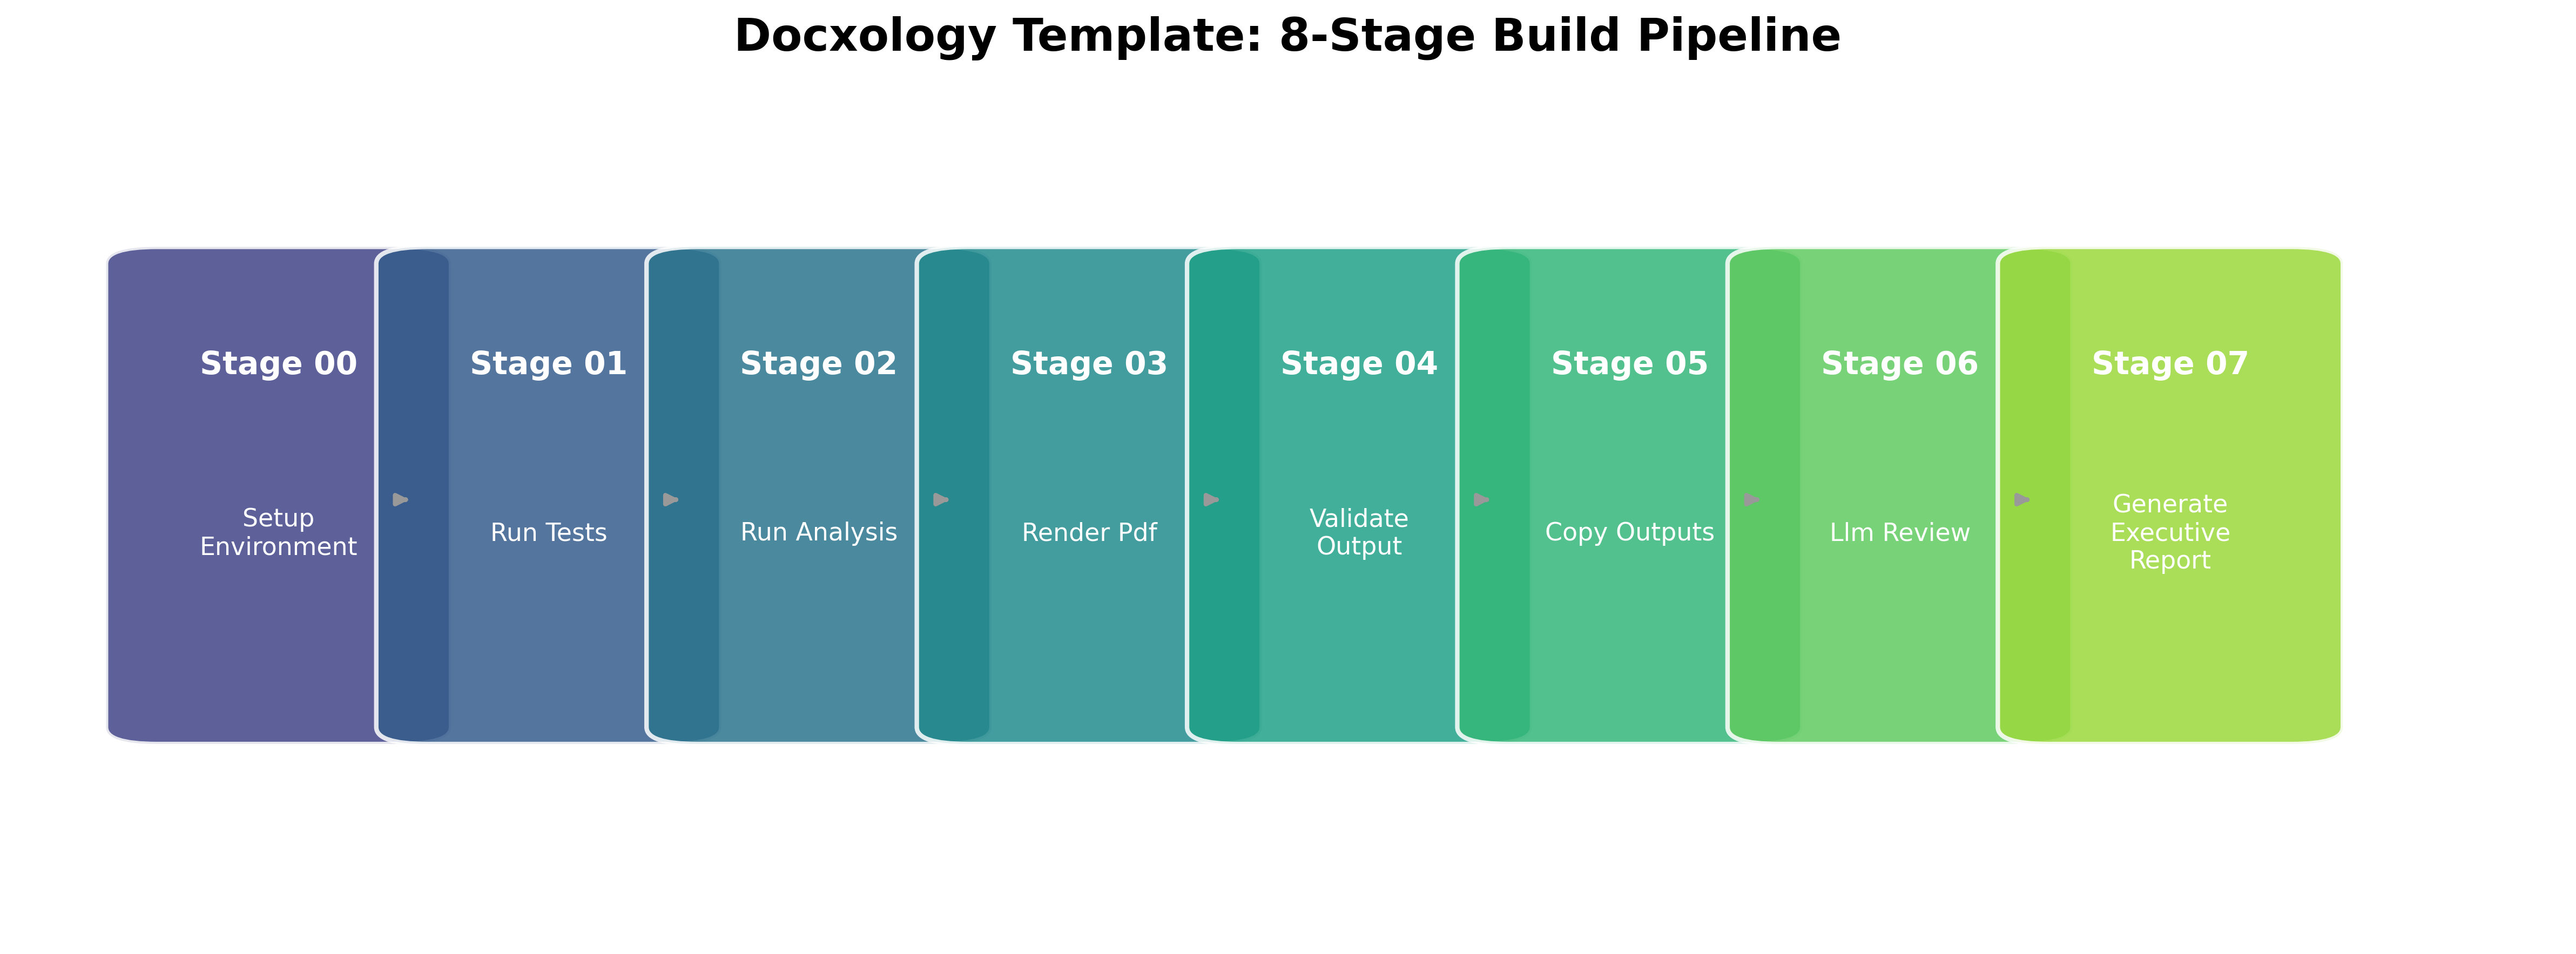
\includegraphics[keepaspectratio,alt={Pipeline Stage Flow}]{../figures/pipeline_stages.png}}
\emph{Figure 2: The eight-stage build pipeline from environment setup
through executive reporting.}

\pandocbounded{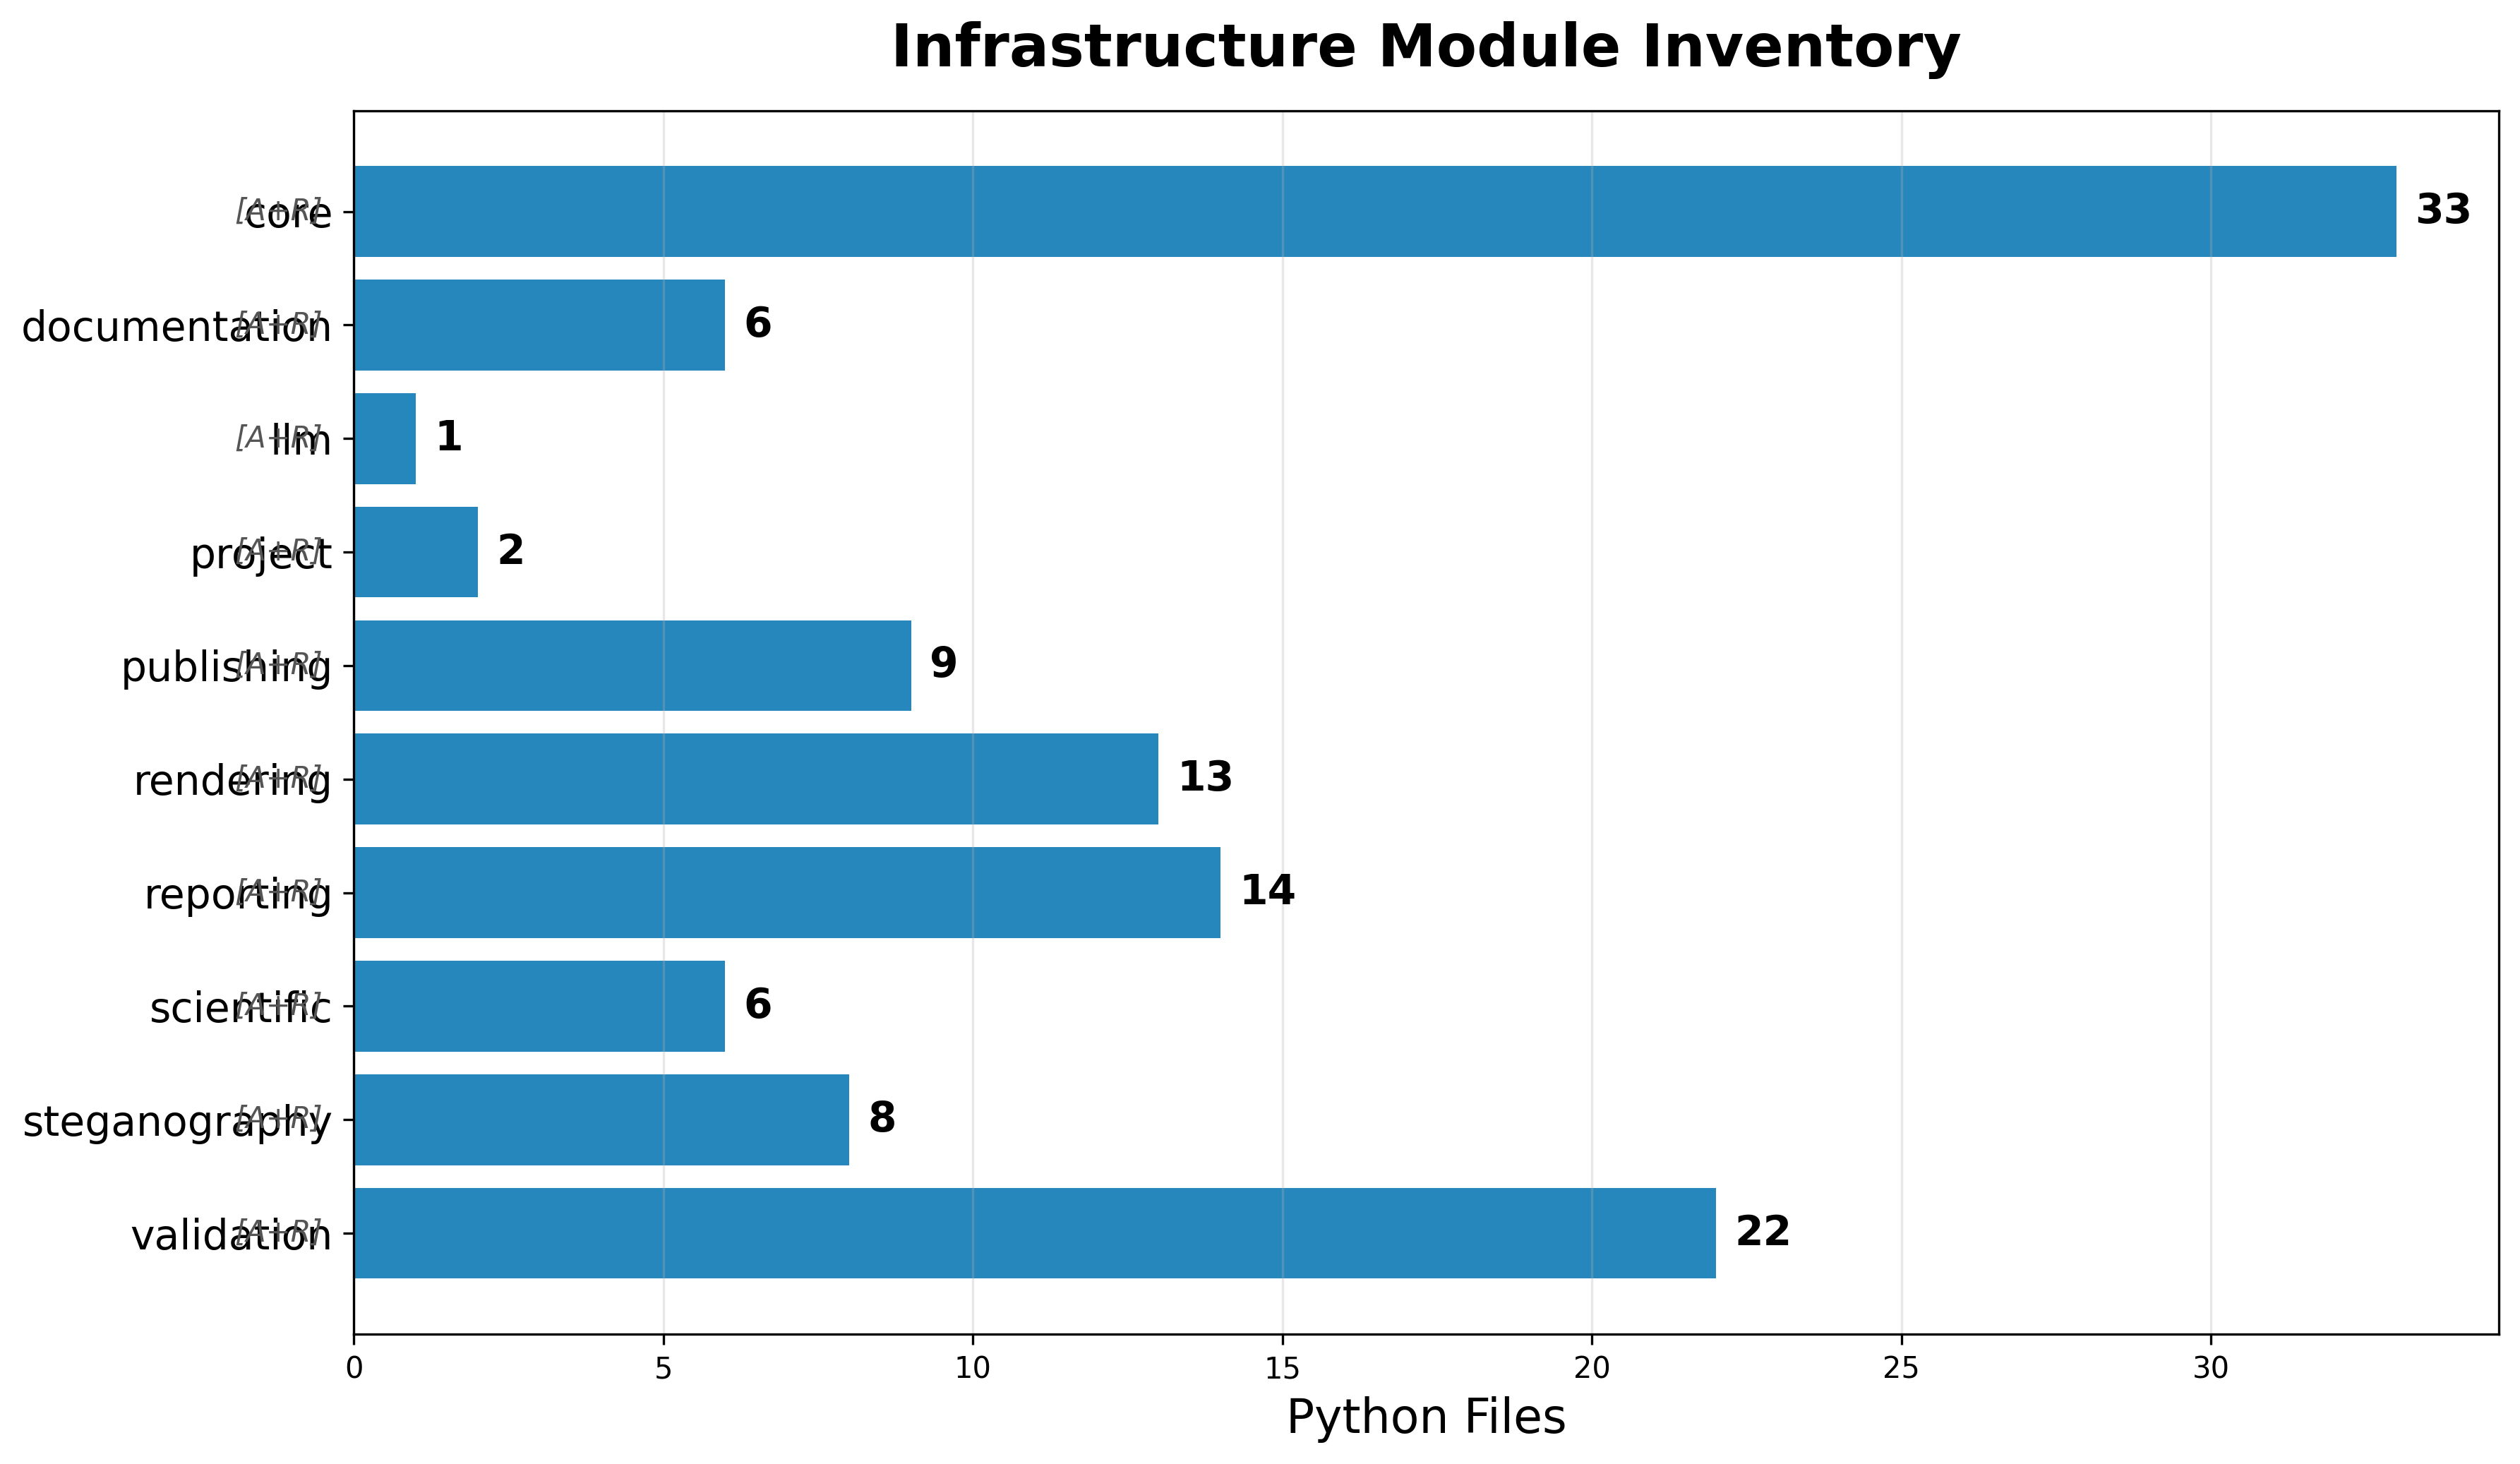
\includegraphics[keepaspectratio,alt={Infrastructure Module Inventory}]{../figures/module_inventory.png}}
\emph{Figure 3: Python file count per infrastructure module, with
documentation status indicators.}
\end{block}

\begin{block}{Comparative Feature Analysis}
\protect\phantomsection\label{comparative-feature-analysis}
To contextualize the Docxology Template's contributions, we compare its
feature set against established tools:

{\def\LTcaptype{none} % do not increment counter
\begin{longtable}[]{@{}
  >{\raggedright\arraybackslash}p{(\linewidth - 12\tabcolsep) * \real{0.1324}}
  >{\centering\arraybackslash}p{(\linewidth - 12\tabcolsep) * \real{0.1618}}
  >{\centering\arraybackslash}p{(\linewidth - 12\tabcolsep) * \real{0.1618}}
  >{\centering\arraybackslash}p{(\linewidth - 12\tabcolsep) * \real{0.1471}}
  >{\centering\arraybackslash}p{(\linewidth - 12\tabcolsep) * \real{0.0735}}
  >{\centering\arraybackslash}p{(\linewidth - 12\tabcolsep) * \real{0.1176}}
  >{\centering\arraybackslash}p{(\linewidth - 12\tabcolsep) * \real{0.2059}}@{}}
\toprule\noalign{}
\begin{minipage}[b]{\linewidth}\raggedright
Feature
\end{minipage} & \begin{minipage}[b]{\linewidth}\centering
Docxology
\end{minipage} & \begin{minipage}[b]{\linewidth}\centering
Snakemake
\end{minipage} & \begin{minipage}[b]{\linewidth}\centering
Nextflow
\end{minipage} & \begin{minipage}[b]{\linewidth}\centering
CWL
\end{minipage} & \begin{minipage}[b]{\linewidth}\centering
Quarto
\end{minipage} & \begin{minipage}[b]{\linewidth}\centering
Jupyter Book
\end{minipage} \\
\midrule\noalign{}
\endhead
Pipeline orchestration & ✓ & ✓ & ✓ & ✓ & --- & --- \\
Manuscript rendering & ✓ & --- & --- & --- & ✓ & ✓ \\
Testing enforcement & ✓ & --- & --- & --- & --- & --- \\
Coverage thresholds & ✓ & --- & --- & --- & --- & --- \\
Cryptographic provenance & ✓ & --- & --- & --- & --- & --- \\
Multi-project management & ✓ & --- & --- & --- & --- & --- \\
AI-agent documentation & ✓ & --- & --- & --- & --- & --- \\
Interactive TUI & ✓ & --- & --- & --- & --- & --- \\
Zero-mock policy & ✓ & --- & --- & --- & --- & --- \\
\bottomrule\noalign{}
\end{longtable}
}

The Docxology Template is, to our knowledge, the only open-source system
that integrates all nine capabilities within a single cohesive
architecture.
\end{block}

\begin{block}{Test Quality Metrics}
\protect\phantomsection\label{test-quality-metrics}
The Zero-Mock testing policy produces measurably higher-fidelity tests:

\begin{itemize}
\tightlist
\item
  \textbf{Zero mock objects} across all test suites (verified by
  automated scanning for \texttt{unittest.mock}, \texttt{MagicMock}, and
  \texttt{patch} imports).
\item
  \textbf{Real filesystem operations}: Tests create, read, validate, and
  delete actual files in temporary directories.
\item
  \textbf{Real subprocess calls}: Pipeline stage tests invoke actual
  \texttt{pytest}, \texttt{pandoc}, and \texttt{xelatex} subprocesses.
\item
  \textbf{Marker-based skip logic}: Tests requiring optional services
  (Ollama, network) use \texttt{@pytest.mark.requires\_ollama} for
  graceful degradation.
\item
  \textbf{Categorical axiom verification}: The
  \texttt{cognitive\_case\_diagrams} project tests validate identity
  morphisms, composition, weight multiplication, and the triangle
  inequality on real enriched category objects.
\end{itemize}
\end{block}
\end{frame}

\end{document}
